\section{Economic Design of the NAX Token}
\subsection{Design goal}
While one of the intentions of the NAX token will be to increase ecosystem activity, the primary design goal is to create a positive reinforcement token economy where all can participate in ecosystem utilization. The core design of a public chain's token economy should conform to certain principles and objectives. These include fair benefits to participants, positive incentives, logical simplicity, and diverse utilization scenarios. 

By creating a token economy with these characteristics, the token naturally has a higher value which thereby promotes the development and expansion of the public chain. A good token economy on a public chain will make the entire ecosystem more dynamic. To sum up, NAX's design goals include:

\begin{enumerate}[\hspace{2cm}(a)]
    \item fair benefits
    \item positive incentives
    \item simple and easy to understand
    \item high utility
    \item smart and effective
\end{enumerate}

\subsection{Core logic}

\subsubsection{Equity fairness and legitimacy}
The effectiveness of a public chain's token economy comes from the fairness and legitimacy of asset acquisition. The requirements for acquiring assets should be simple, transparent and an identical process for the vast majority of people. In a public token economy, the assets owned are relatively fair and substantiated - due to this, the primary way to obtain equity of a token via a pledging (Staking) method is in line with the above requirements. Equity obtainment must not be due to requirements not clear or loopholes existing which lead to the phenomenon of poor asset allocation - the overall result of obtainment must be conducive to improved ecosystem development on the public chain.

Within the Nebulas ecosystem, the pledging (Staking) process of NAS to obtain the benefits of NAX is fair and equitable within the Nebulas Eco-Certified economy.

\subsubsection{Nebulas smart pledge}
Traditionally, the pledge method used requires users to transfer their assets into smart contracts for temporary custody and asset security is controlled within in the smart contract. Unfortunately, history of smart contract asset security issues is not uncommon. For example, in 2016, the DAO project on Ethereum was comprimised and attackers used contract loopholes and caused a huge economic losses for investors and made them doubt the safety of smart contracts. Due to this, pledging also puts great pressure onto the public chain project parties since a large number of assets are kept in a smart contract which makes them targets; making the management and security of the smart contract a very big development bottleneck. All assets on the blockchain are genuine and pledging simply locks in the liquidity of that asset - it does not validate the ownership of the asset (although it can be retrieved by calling the contract method) once transferred to the contract.

For NAX asset obtainment via staking, we propose a new mechanism entitled "Nebulas Smart Staking" which records the locking of liquidity via smart contract between the Nebulas address owner and the pledge contract while ensuring the user's assets are still owned by the user. The role of the pledge contract is to simply verify the validity of the user's pledge by randomly checking the on-chain contract status and the pledging address. A  pledge is considered valid when the balance of the pledging address is equal or greater to the amount pledged to the smart contract.

The advantages of the Nebula Smart Pledge include:
\begin{enumerate}[\hspace{2cm}(a)]
    \item guarantees the user's asset identification
    \item motivates more users to participate in pledge
    \item asset security decentralization
    \item Asset Securitization and Separation of Asset Liquidity
\end{enumerate}

\subsubsection{NAX Extended Model - NDM}
As mentioned above, on the basis of safeguarding the equity and legitimacy of assets, and ensuring the inviolable ownership of pledged assets, the user contributes the liquidity of their assets to obtain the corresponding ecological rights and interests. We call this new mode of token issuance NDM (Nebulas Devotional Mining). 

The maximum amount of NAX tokens projected to be released is 10 billion(\(10^{10}\)) with an issuance cycle of every 6,000 blocks (approximately once per day tokens will be distributed). The number of tokens issued per cycle decreases with an attenuation coefficient of $\mu=0.999$ which leads to distribution completion in about 12 years. The number of pre-issued NAX changes with the number of cycles\ref{dist}, and the cumulative pre-issued NAX number is shown in \ref{acc}.

\begin{figure}
\centering
    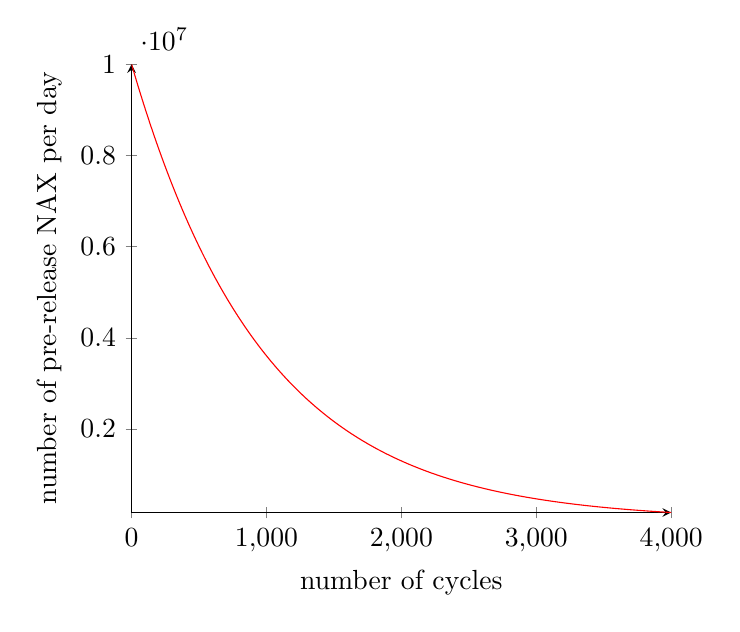
\begin{tikzpicture}
    \begin{axis}[
        axis lines = left,
        xlabel = {number of cycles},
        ylabel = {number of pre-release NAX per day},
    ]
    \addplot [
        domain=-0:4000, 
        samples=1000,
        color=red,
    ]
    {1.0*10^7*0.999^x};

    \end{axis}
    \end{tikzpicture}
    \caption{Daily pre-release NAX number and period relationship}\label{dist}
\end{figure}


% cumulative number of issued NAX and periodic relationship
\begin{figure}
\centering
    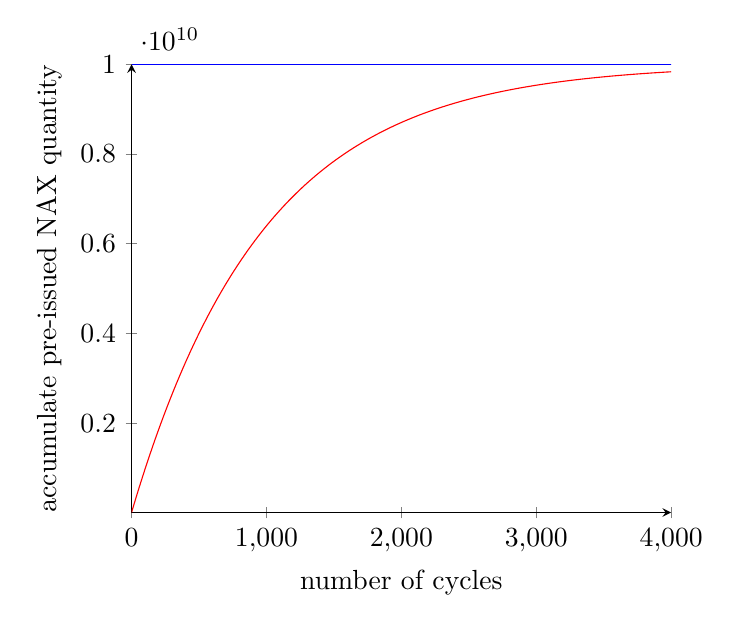
\begin{tikzpicture}
    \begin{axis}[
        axis lines = left,
        xlabel = {number of cycles},
        ylabel = {accumulate pre-issued NAX quantity},
    ]
    \addplot [
        domain=-0:4000, 
        samples=1000, 
        color=red,
    ]
    {10^10*(1 - 0.999^(x+1))};

    \addplot [
        domain=-0:4000, 
        samples=1000, 
        color=blue,
    ]
    {10^10};
    \end{axis}
    \end{tikzpicture}
\caption{Accumulate pre-issued NAX quantity and period relationship}\label{acc}
\end{figure}

\subsubsection{Dynamic Distribution Model}
The so-called dynamic distribution model means that on the basis of pre-issuance, some variables will be introduced to promote the positive ecosystem growth. During the initial stage of NAX, we will introduce multiple variables which will control distribution such as pledge rate influence factor and a dynamically adjusted  distribution ratio based on the to the rise and fall (quantity) of pledged assets. Any undistributed NAX for a cycle will be rolled over to the following cycle for greater distribution based on the variables. As needed in the future, we will also introduce a more dynamic distribution model.

Therefore, for each period of $i$, the system will pre-issue $C_i$ NAX assigned to the user currently being pledged. When the system distributes, it will determine a distribution coefficient $\lambda_i$ based on the current pledge rate level r (the total amount of pledge NAS currently involved / total NAS circulation), and actually distribute $C_i$$\lambda_i$ (0< $\lambda_i$<1) NAX. Remaining undistributed $C_i$(1 - $\lambda$) NAX will roll over which in turn increases the total amount of pre-issued tokens for the following cycle. Therefore, the \(i\) period issuance pool, \(C_i = C_0 \mu^i + C_{i-1} (1-\lambda_{i-1})\), consists of two parts: The first part is the basic part, and each period is continuously attenuated with an attenuation coefficient of $\mu$. The second part is the remainder of the previous issuance pool.

Among them, the distribution coefficient \(\lambda_i\) and the pledge rate \(r_i\) function relationship as shown in the following formula. For specific parameters, please refer to the appendix. The function relationship is shown in \ref{func}.

  \begin{equation}
    \lambda_i = l r_i^3 + m r_i^2 + n r_i
  \end{equation}

\begin{figure}
\centering
    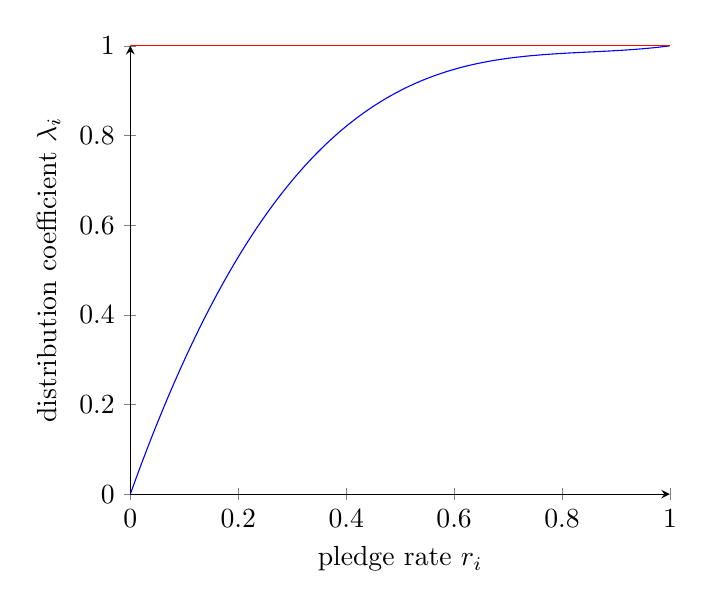
\begin{tikzpicture}
    \begin{axis}[
        axis lines = left,
        xlabel = {pledge rate $r_i$},
        ylabel = {distribution coefficient $\lambda_i$},
    ]
    \addplot [
        domain=0:1,
        samples=100,
        color=blue,
    ]
    {1.52*x^3-3.88*x^2+3.36*x};
    \addplot [
        domain=-0:1, 
        samples=100, 
        color=red,
    ]
    {1};
    \end{axis}
    \end{tikzpicture}
    \caption{Relationship between distribution coefficient and pledge rate}\label{func}
\end{figure}



\subsubsection{Distribution model in cycle}
During a distribution cycle, different number of pledge cycles will result in different distribution weights. The system determines the final NAX distribution amount based on the pledge quantity of each pledged user $V_{i, j}$ and the pledge weight \(f(T_{i, j})\). If the $N$ address is validly pledging (retaining enough assets) during the $i$ period, the $j$ address pledge is $V_{i,j}$ and the effective pledge period is $T_{i,j}$. Therefore, the number of NAXs that the address can be distributed to is $K_{i,j}$ as shown in the following formula.

\begin{equation}
  K_{i,j} = \frac{V_{i,j} f(T_{i,j})}{\sum_j V_{i,j} f(T_{i,j})} \lambda_i C_i
\end{equation}



Where \(f(T_{i,j})\) is the effective weight function for the pledge of the \(i\) user\(j\). The relationship between the pledge weight and the number of pledge cycles is as follows, where the function relationship is shown in \ref{weight}.
  \begin{equation}
    f(T) = 1 - \frac{\sqrt{(aT+b)^2+c^2}-(aT+b)}{2}
  \end{equation}

The parameters $a$, $b$, $c$, etc... in the formula are discussed in the appendix. In general, within the same cycle, the system allocates the total amount of additional issuance tokens according to the number of pledges and the corresponding length of the pledge. In order to achieve a fair result, the more pledges and the longer the pledge, the higher the issuance number will be. At the same time, this method makes new pledge users more motivated and the existing users' weight will be retained at a considerable level. The design will reach the following scenarios:

\begin{enumerate}[\hspace{1cm}(a)]
  \item Early users involved in pledge have a greater probability of receiving more issuance
  \item As the pledge rate increases, the number of system issuance will increase accordingly to encourage more people to join the pledge.
\end{enumerate}

\begin{figure}
\centering
    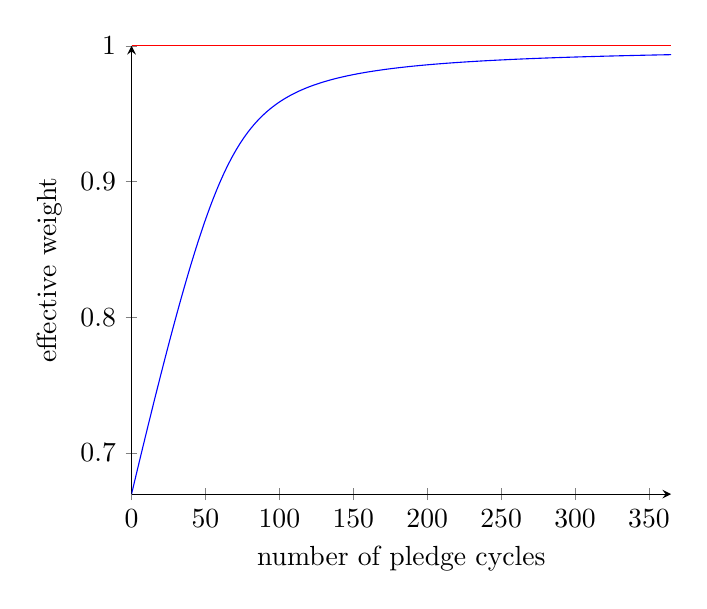
\begin{tikzpicture}
    \begin{axis}[
        axis lines = left,
        xlabel = {number of pledge cycles},
        ylabel = {effective weight},
    ]
    \addplot [
        domain=0:365,
        samples=200,
        color=blue,
    ]
    {1-(sqrt((0.005*x-0.3)^2+0.2^2)-(0.005*x-0.3))/2};

    \addplot [
        domain=-0:365, 
        samples=200, 
        color=red,
    ]
    {1};
    \end{axis}
    \end{tikzpicture}
    \caption{Relationship between the effective weight of the pledge and the number of pledge cycles}\label{weight}
\end{figure}

\subsubsection{Foundation Fees}
In order to enable the Nebulas Foundation to have more abilities and initiative in ecosystem investment, incubation, support, activities, etc..., the additional issuance of $5\%$ will be transferred to NAX. The addresses managed by the foundation are subject to public scrutiny as well as its usage. The specific contents will be disclosed in the future.


\subsection{Contract Framework}
NAX is an extensible NRC20 contract consisting of a set of contracts which manage data and parameters of the entire contract via multi-sign contracts as shown in detail in \ref{fig:nax_framework}.

\begin{figure}[htbp]
  \centering
    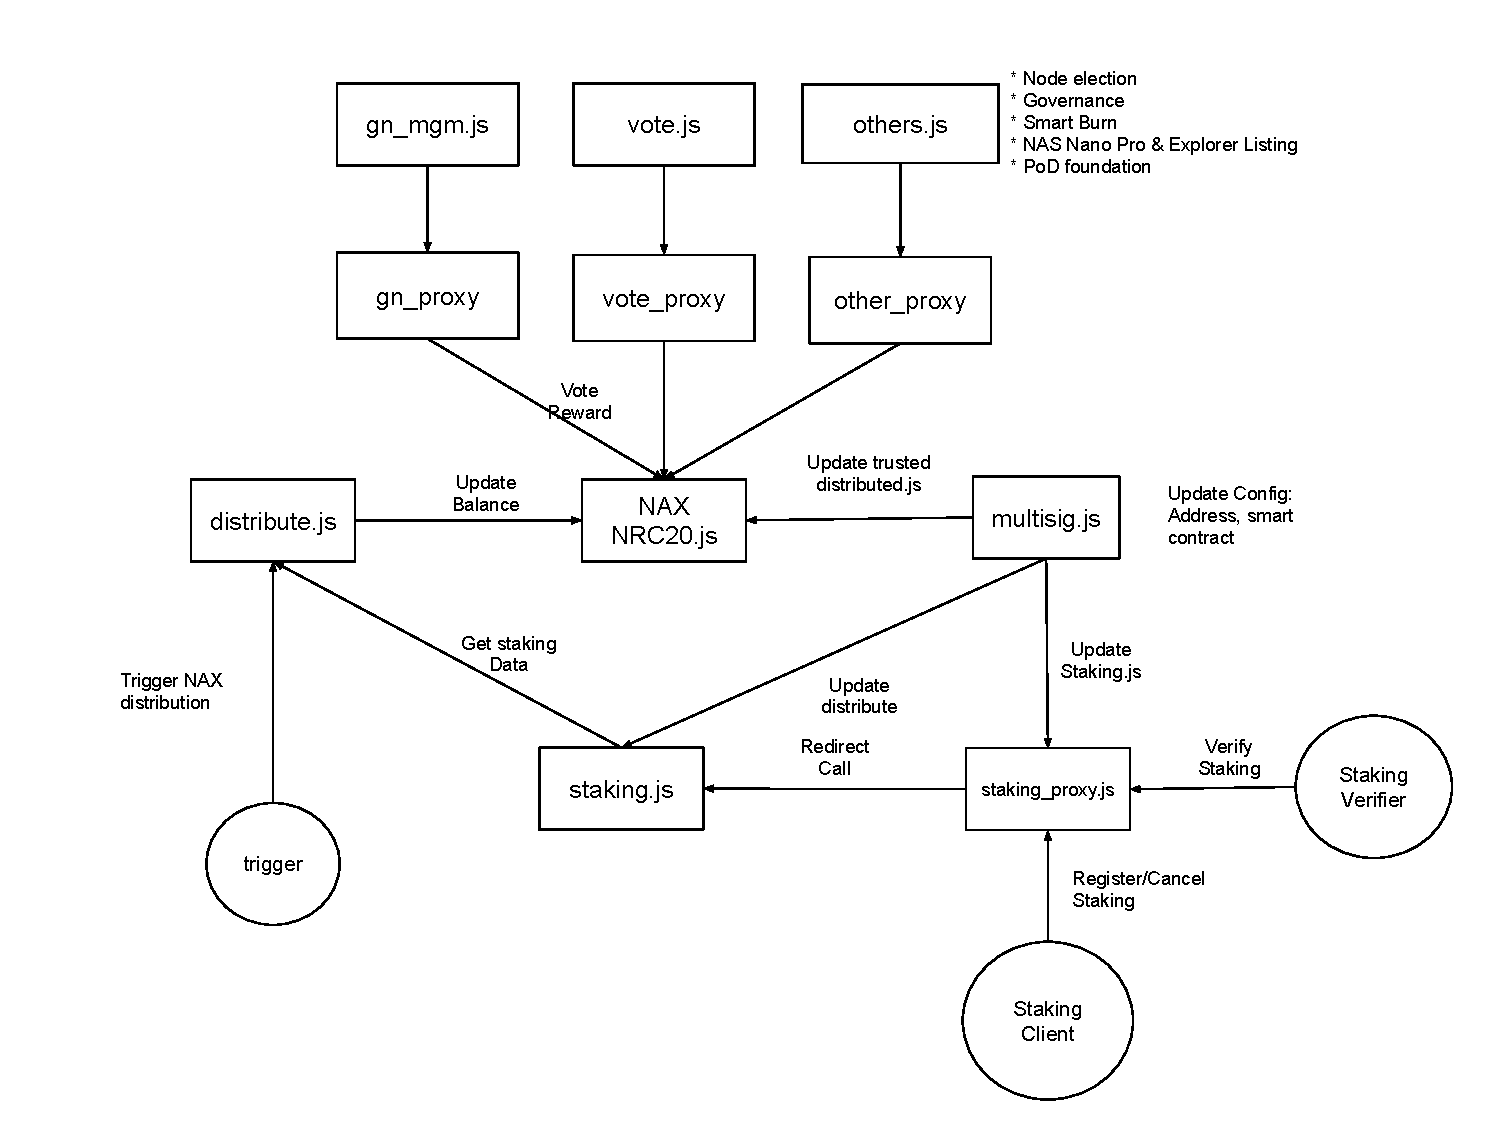
\includegraphics[width=1\textwidth]{../common/nax.pdf}
    \caption{NAX contract component schematic \label{fig:nax_framework}}
\end{figure}
